\documentclass[ 12pt ]{article}
\usepackage{amsmath, amsthm, amssymb, csquotes, enumitem, graphicx, listings, mathrsfs}
\usepackage[margin=0.5in]{geometry}
\graphicspath{ ./ }

\begin{document}

\begin{titlepage}
    \begin{center}
        \vspace*{1cm}
            
        \LARGE
        \textbf{CS 479 Pattern Recognition}

        \vspace{0.5cm}
        \LARGE
        \textbf{Programming Assignment 1}

        \vspace{0.1cm}
        \LARGE
        \textbf{Bayesian Decision Theory}
            
        \vspace{1.5cm}
            
        \textbf{Logan Leavitt \& Landon Fox}
            
        \vfill
        \Large
        \textbf{Collaboration}

        \vspace{0.1cm}
        \large
        For the implementation, both Logan and Landon contributed. Logan carried out the Bayesian Classifier, the skin-color methodology, and most debugging. Landon worked on the
        file and image input/output as well as parameter estimation. Together we collaborated on the ROC curves. \\
        In regard to the report, Logan worked on the Results, formatting, and grammar. Landon contributed to the Theory and Implementation.
            
        \vspace{0.8cm}
            
            
        \Large
        University of Nevada Reno\\
        April 12, 2021
            
    \end{center}
\end{titlepage}


\section*{Theory}

When attempting to apply Bayesian Decision Theory to a decision problem, that is, attempting to classify a feature $\textbf{x}$ into classes $\omega_1, \hdots, \omega_c$ via Bayes Rule
$$P(\omega_j \mid \textbf{x}) = \frac{p( \textbf{x} \mid \omega_j ) P(\omega_j)}{p(\textbf{x})},$$ we are provided the task of estimating $P(\omega_j)$ and $p(\textbf{x} \mid \omega_j)$.
Generally, it can be quite easy to estimate $P(\omega_j)$, it is far more of a challenge to obtain $p(\textbf{x} \mid \omega_j)$. To approach this problem, we will make the following assumptions:
\begin{itemize}
    \item We have a set $D_j$ of $n_j$ independently drawn samples belonging to the distribution $p(\textbf{x} \mid \omega_j)$ for each $1 \leq j \leq c$.
    \item The distribution $p(\textbf{x} \mid \omega_j)$ can be modeled as a Gaussian Distribution $N(\boldsymbol{\mu}, \Sigma)$ for all classes $\omega_j$.
\end{itemize}
The latter of the assumptions is quite a strong restriction and may not always apply and so we must apply this only when we believe the underlying distribution is truly Gaussian.
Now, our goal is to estimate a $\boldsymbol{\theta}_j = ( \boldsymbol{\mu}_j, \Sigma_j )$ for each class to \textit{best} suit our distribution. Through the lens of Maximum Likelihood
Estimation, we can view $\boldsymbol{\theta}_j$ as a fixed point that we will adjust such that the probability of our samples occurring is maximized. Furthermore, $$\hat{\boldsymbol{\theta}}_j
= \underset{\boldsymbol{\theta}_j}{\arg \max}\, p(D_j \mid \boldsymbol{\theta}_j)$$ is our desired result. Provided independently drawn samples, we may assume that $$p(D_j \mid \boldsymbol{\theta}_j)
= p( \textbf{x}_1, \hdots, \textbf{x}_{n_j} \mid \boldsymbol{\theta}_j) = \prod_{k = 1}^{n_j} p(\textbf{x}_k \mid \boldsymbol{\theta}_j)$$ and further simplify via a logarithm $$\ln p(D_j \mid
\boldsymbol{\theta}_j) = \sum_{k = 1}^{n_j} \ln p(\textbf{x}_k \mid \boldsymbol{\theta}_j)$$ allowing us to maximize $$\hat{\boldsymbol{\theta}}_j = \underset{\boldsymbol{\theta}_j}{\arg \max}\,
\ln p(D_j \mid \boldsymbol{\theta}_j)$$ for less computational cost.

To solve this optimization problem, we may utilize multivariate calculus. Moreover, when solving for $(\hat{\boldsymbol{\mu}}_j, \hat{\Sigma}_j)$ by calculating the total derivative of our objective function and setting the
result equal to zero, we obtain the sample mean and sample covariance, $$\hat{\boldsymbol{\mu}}_j = \frac{1}{n_j} \sum_{k = 1}^{n_j} \textbf{x}_k\;\;\; \mathrm{and}\;\;\; \hat{\Sigma}_k =
\frac{1}{n_j} \sum_{k = 1}^{n_j} ( \textbf{x}_k - \hat{\boldsymbol{\mu}} )( \textbf{x}_k - \hat{\boldsymbol{\mu}})^t,$$ a fundamental result of Maximum Likelihood Estimation.

\section*{Implementation}

To implement Parameter Estimation, all we must do is calculate the sample mean and covariance from a sample of our distribution. In the file \verb|ParameterEstimation.h|, we make use of
the \verb|Armadillo| Linear Algebra library to calculate both parameters when provided a \verb|std::vector| of distribution samples. To make use of the parameters and classify provided
features, we modified our existing dichotomic Bayesian Classifier, implemented under \verb|BayesianClassifier.h|, with accordance to \verb|Armadillo|. In practice, we first gather all
data from our distribution using file input/output, \verb|FileIO.h|, estimate both the mean and covariance for our distributions, place the results into a \verb|Category| which is
then given to a Bayesian Classifier. Then we iterate through our features, classifying them and accounting for all misclassifications.

In regard to the skin-color methodology, we had followed the approach of Yang et al. by utilizing the chromatic color space and training our Bayesian Classifier with the provided image
\verb|Training_1.ppm| and the properly classified image \verb|ref1.ppm|. The discriminant is implemented as the probability density function without the normalizing factor. That is, the discriminant function is $g(x)= e^{-\frac{1}{2}(x - \mu)^t \Sigma^{-1} (x - \mu)}$.
Then to test our model, we performed a classification on \verb|Training_3.ppm| and \verb|ref1.ppm| as well as
\verb|Training_6.ppm| and \verb|ref6.ppm|. There we make use of \verb|Image.h| to handle image input/output.

\section*{Results}

\begin{enumerate}
    \item[\textbf{1.}] $ $
        \begin{enumerate}
                \item[\textbf{a.}] As implemented in \verb|problem1a.cpp|, we begin by estimating the parameters $(\hat{\boldsymbol{\mu}}_1, \hat{\Sigma}_1)$ and $(\hat{\boldsymbol{\mu}}_2, \hat{\Sigma}_2)$ provided all 200,000 samples drawn from the distributions $N(\boldsymbol{\mu}_1, \Sigma_1)$ and $N(\boldsymbol{\mu}_2, \Sigma_2)$, respectively, where $$\boldsymbol{\mu}_1 = \begin{bmatrix} 1 \\ 1
\end{bmatrix},\; \Sigma_1 = \begin{bmatrix} 1 & 0 \\ 0 & 1 \end{bmatrix},\;\;\; \boldsymbol{\mu}_2 = \begin{bmatrix} 4 \\ 4 \end{bmatrix},\; \Sigma_2 = \begin{bmatrix} 1 & 0 \\ 0 & 1 \end{bmatrix}.$$ After classifying all results into the file \verb|output1a-1.csv|, we obtain a total misclassification rate of 1.5485\% with an error rate of 0.82800\% and 0.7205\% from class one and two, respectively. Observe Table 1 below. Our results using the true mean and covariance provided a total error of 1.5485\% with a misclassification rate of 0.8295\% and 0.7190\% from class one and two, respectively. Observe that our error rate utilizing the estimated parameters is almost exactly that of the error rate achieved using the true parameters. For estimated parameters, see Table 2.

                \item[\textbf{b.}] Now, we repeat the same experiment using only 0.01\%, 0.1\%, 1\%, and 10\% of the samples. Additionally, we will experiment with the use of explicitly masking our covariance matrices as diagonal similar to the original covariance matrix used to create the distributions. We obtain the following results
\begin{center}
                
                \begin{tabular}{|l|lll|lll|}
                    \hline
                    & \multicolumn{3}{l|}{Misclassification Rates \%} & \multicolumn{3}{l|}{Error Rates with Diagonal Covariance \%} \\
                    Sample Sizes & Class 1 & Class 2 & Total & Class 1 & Class 2 & Total \\
                    \hline
                    True Distribution & 0.8295 & 0.719 & 1.5485 & 0.8295 & 0.719 & 1.5485 \\
                    100\% & 0.8280 & 0.7205 & 1.5485 & 0.8255 & 0.7240 & 1.5495 \\
                    10\% & 0.8450 & 0.8100 & 1.6550 & 0.8350 & 0.8100 & 1.6450 \\
                    1\% & 0.9000 & 0.6500 & 1.5500 & 0.9000 & 0.7000 & 1.6000 \\
                    0.1\% & 0.000 & 1.5000 & 1.500 & 0.0000 & 2.0000 & 2.0000 \\
                    0.01\% & 0.0000 & 5.0000 & 5.0000 & 0.0000 & 5.0000 & 5.0000 \\
                    \hline
                \end{tabular}
        \scriptsize
                    Table 1: The misclassification rates of the Bayesian Classifier provided estimated parameters of varying sample sizes as well as diagonal covariance matrices.
\end{center}

\begin{center}
                
                \begin{tabular}{|l|llll|}
                    \hline
                    & \multicolumn{4}{l|}{Parameters} \\
                    Sample Sizes & Class 1 Mean & Class 1 Covariance & Class 2 Mean & Class 2 Covariance \\
                    \hline
                    True Dist. & $\begin{bmatrix} 1 \\ 1 \end{bmatrix}$ & $\begin{bmatrix} 1 & 0 \\ 0 & 1 \end{bmatrix}$ & $\begin{bmatrix} 4 \\ 4 \end{bmatrix}$ & $\begin{bmatrix} 1 & 0 \\ 0 & 1 \end{bmatrix}$ \\
                    100\%  & $\begin{bmatrix} 0.9950 \\ 1.0019 \end{bmatrix}$ & $\begin{bmatrix} 1.0092 & -0.0040 \\ -0.0040 & 0.9983 \end{bmatrix}$ & $\begin{bmatrix} 3.9979 \\ 4.0046 \end{bmatrix}$ & $\begin{bmatrix} 0.9983 &  0.0007 \\  0.0007 & 0.9988 \end{bmatrix}$ \\
                    10\%   & $\begin{bmatrix} 0.9976 \\ 1.0268 \end{bmatrix}$ & $\begin{bmatrix} 0.9845 & -0.0085 \\ -0.0085 & 0.9801 \end{bmatrix}$ & $\begin{bmatrix} 4.0038 \\ 4.0135 \end{bmatrix}$ & $\begin{bmatrix} 0.9949 & -0.0031 \\ -0.0031 & 0.9878 \end{bmatrix}$ \\
                    1\%    & $\begin{bmatrix} 0.9809 \\ 1.0454 \end{bmatrix}$ & $\begin{bmatrix} 1.0207 & -0.0163 \\ -0.0163 & 0.8974 \end{bmatrix}$ & $\begin{bmatrix} 3.9462 \\ 3.9888 \end{bmatrix}$ & $\begin{bmatrix} 1.0034 &  0.0425 \\  0.0425 & 0.9834 \end{bmatrix}$\\
                    0.1\%  & $\begin{bmatrix} 1.0403 \\ 1.0540 \end{bmatrix}$ & $\begin{bmatrix} 0.8067 & -0.1094 \\ -0.1094 & 0.7880 \end{bmatrix}$ & $\begin{bmatrix} 3.9076 \\ 4.1094 \end{bmatrix}$ & $\begin{bmatrix} 1.1556 &  0.1026 \\  0.1026 & 1.0663 \end{bmatrix}$\\
                    0.01\% & $\begin{bmatrix} 1.2703 \\ 0.9113 \end{bmatrix}$ & $\begin{bmatrix} 0.2568 & -0.0178 \\ -0.0178 & 0.6775 \end{bmatrix}$ & $\begin{bmatrix} 3.5043 \\ 3.8515 \end{bmatrix}$ & $\begin{bmatrix} 1.7761 & -0.3529 \\ -0.3529 & 0.8295 \end{bmatrix}$\\
                    \hline
                \end{tabular}
                \scriptsize
                    Table 2: The estimated parameters used in classification.
                \end{center}


        \end{enumerate}

    \item[\textbf{2.}] $ $
        \begin{enumerate}
            \item[\textbf{a.}] The experiment from 1(a) is repeated, except with samples from different distributions. The new distributions are given by $N(\boldsymbol{\mu}_1, \Sigma_1)$ and $N(\boldsymbol{\mu}_2, \Sigma_2)$, where $$\boldsymbol{\mu}_1 = \begin{bmatrix} 1 \\ 1
\end{bmatrix},\; \Sigma_1 = \begin{bmatrix} 1 & 0 \\ 0 & 1 \end{bmatrix},\;\;\; \boldsymbol{\mu}_2 = \begin{bmatrix} 4 \\ 4 \end{bmatrix},\; \Sigma_2 = \begin{bmatrix} 4 & 0 \\ 0 & 8 \end{bmatrix}.$$ After classifying all results into the file \verb|output2a-1.csv|, we obtain a total misclassification rate of 6.109\% with an error rate of 0.962\% and 5.147\% from class one and two, respectively. Our results using the true mean and covariance provided a total error of 6.987\% with a misclassification rate of 2.746\% and 4.241\% from class one and two, respectively. Interestingly, the error rate for the Maximum likelihood classification is lower than that of the true Bayesian Classifier. This could be due to Maximum Likelihood estimation overfitting the sampled data.

            \item[\textbf{b.}] Using the same distributions from 2(a), we repeat the experiment from 1(b) by sampling various sizes of data. Additionally, the same experiment was run while forcing the covariance matrices to be diagonal. The results are contained in Table 2.
\begin{center}
                
                \begin{tabular}{|l|llll|}
                    \hline
            & \multicolumn{4}{l|}{Parameters for 2(b)} \\
                    True Dist. & $\begin{bmatrix} 1 \\ 1 \end{bmatrix}$ & $\begin{bmatrix} 1 & 0 \\ 0 & 1 \end{bmatrix}$ & $\begin{bmatrix} 4 \\ 4 \end{bmatrix}$ & $\begin{bmatrix} 4 & 0 \\ 0 & 8 \end{bmatrix}$ \\
                    100\% & $\begin{bmatrix} 1.0043 \\ 0.9940 \end{bmatrix}$ & $\begin{bmatrix} 1.0002 & 0.0068 \\  0.0068 & 1.00541 \end{bmatrix}$ & $\begin{bmatrix} 4.0029 \\ 3.9800 \end{bmatrix}$ & $\begin{bmatrix} 16.083 & -0.0103 \\ 0.0103 & 64.1359 \end{bmatrix}$ \\
                    1\% & $\begin{bmatrix} 1.0013 \\ 0.9627 \end{bmatrix}$ & $\begin{bmatrix} 1.021293 & 0.0082 \\ 0.0082 & 1.0569 \end{bmatrix}$ & $\begin{bmatrix} 3.8458 \\ 4.2380 \end{bmatrix}$ & $\begin{bmatrix} 15.9150 & -0.8493 \\ -0.8493 & 64.8413 \end{bmatrix}$\\
                    0.1\% & $\begin{bmatrix} 1.1310 \\ 1.2340 \end{bmatrix}$ & $\begin{bmatrix} 0.7655 & -0.0925 \\ -0.0925 & 1.1366 \end{bmatrix}$ & $\begin{bmatrix}  4.0143 \\ 3.4371 \end{bmatrix}$ & $\begin{bmatrix} 15.2832 & -4.3572 \\ -4.3572 & 74.2259 \end{bmatrix}$\\
                    0.01\% & $\begin{bmatrix} 1.0143 \\ 1.0358 \end{bmatrix}$ & $\begin{bmatrix} 0.2390 & 0.1575 \\ 0.1575 & 1.1693 \end{bmatrix}$ & $\begin{bmatrix}  4.0143 \\ 3.4372 \end{bmatrix}$ & $\begin{bmatrix} 15.2832 & -4.3573 \\ -4.35727 & 74.2259 \end{bmatrix}$\\
         \hline
                \end{tabular}
                \newline
                \scriptsize
                    Table 3: The estimated parameters used in classification.
                \end{center}
        \end{enumerate}

    \item[\textbf{3.}]
        \begin{enumerate}
                    \item[\textbf{a.}] The performance of this classification method is tested on \verb|Training_3.ppm| and \verb|Training_6.ppm| by using the probability distribution obtained from \verb|Training_1.ppm|. The optimal threshold is obtained by testing 20 uniformly distributed values from 0 to 1 $(0, 0.05, 0.1, 0.15, \hdots)$. Figures 1 and 2 show the results obtained.
\begin{center}
    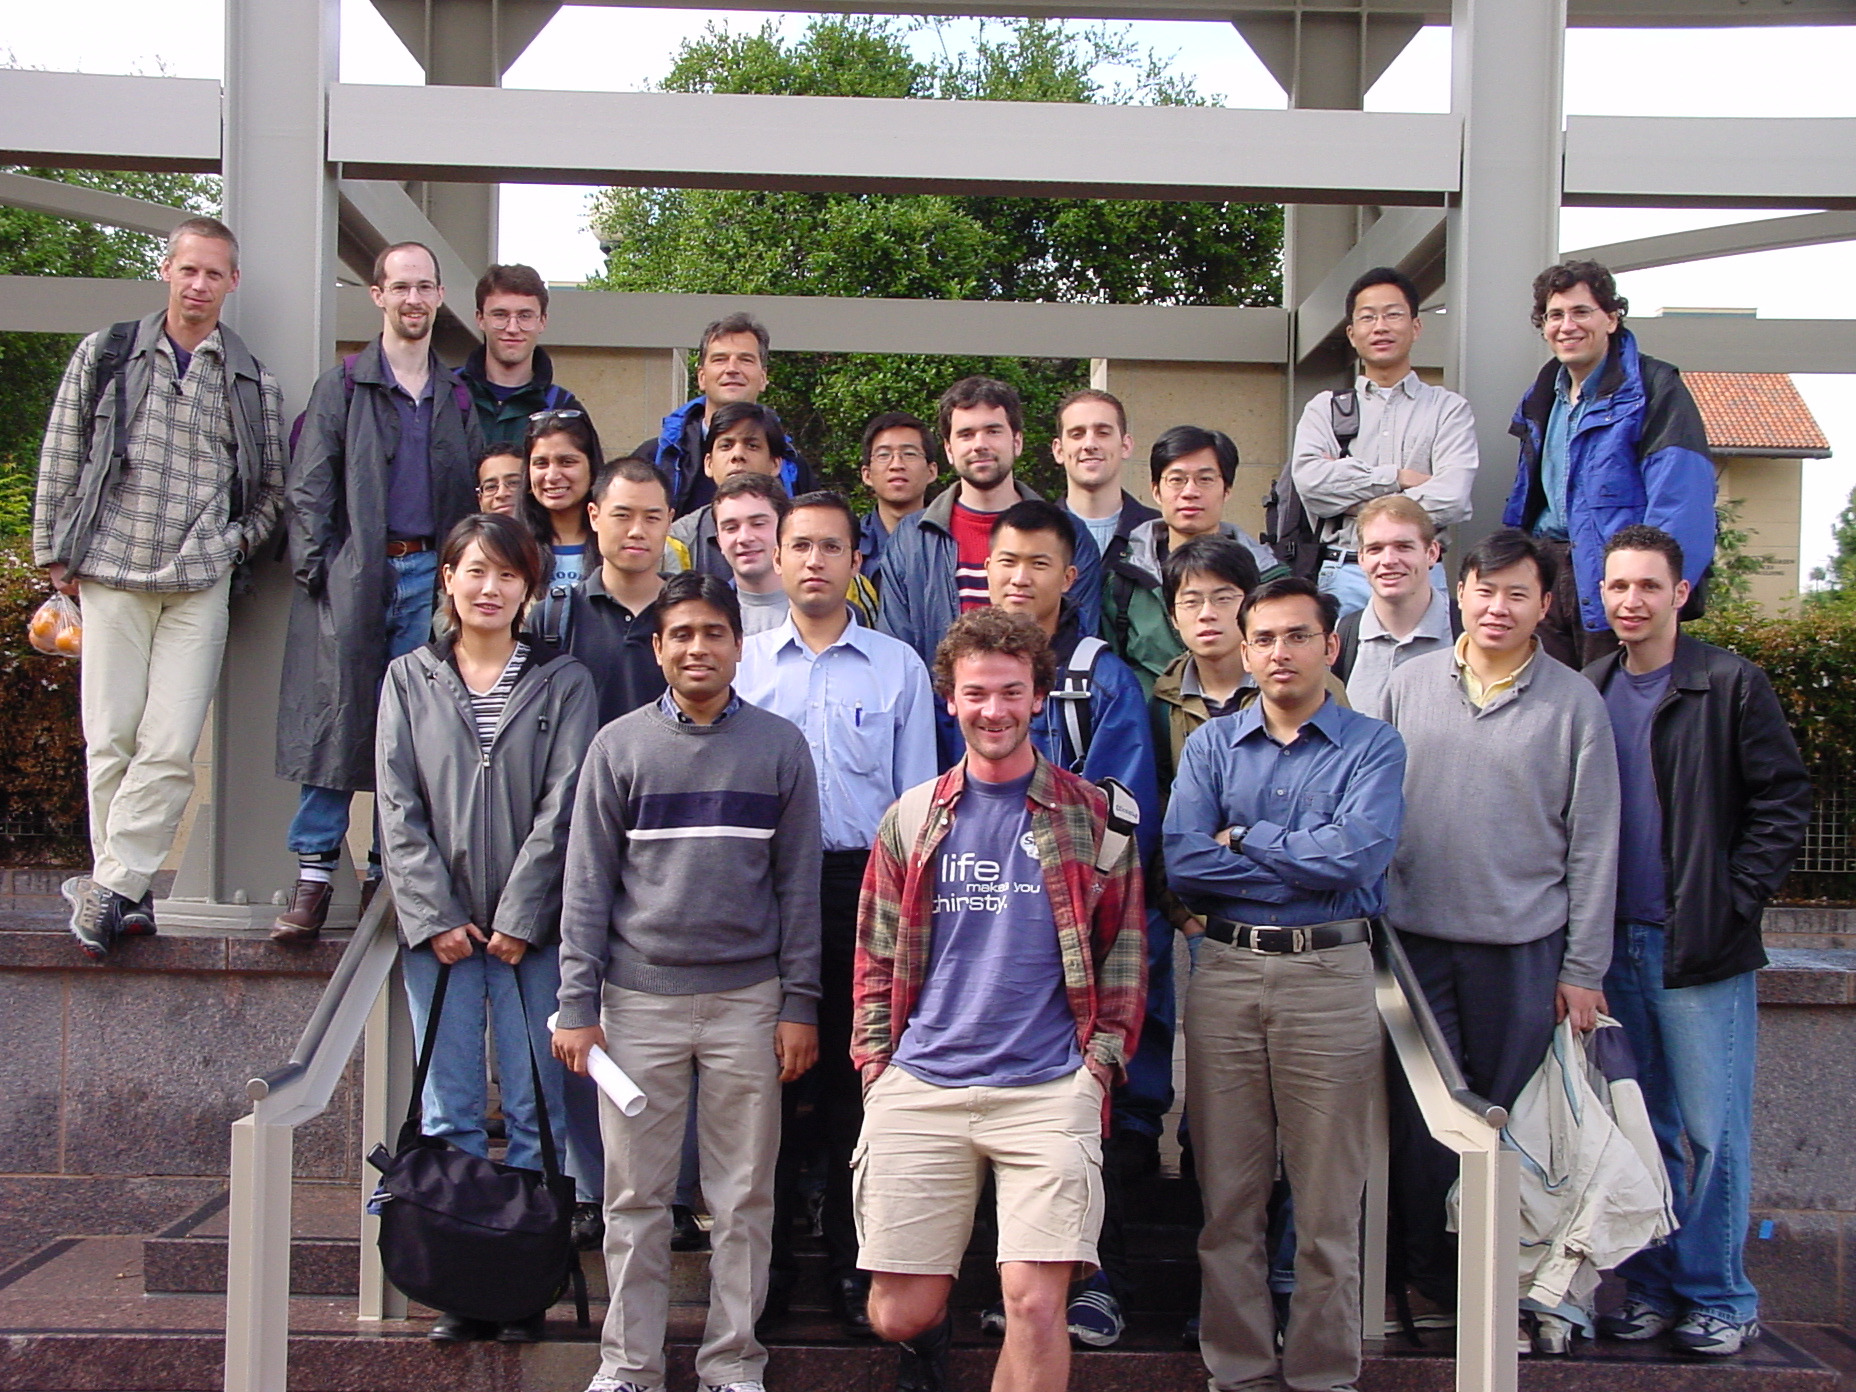
\includegraphics[scale=0.1]{Training_3}
    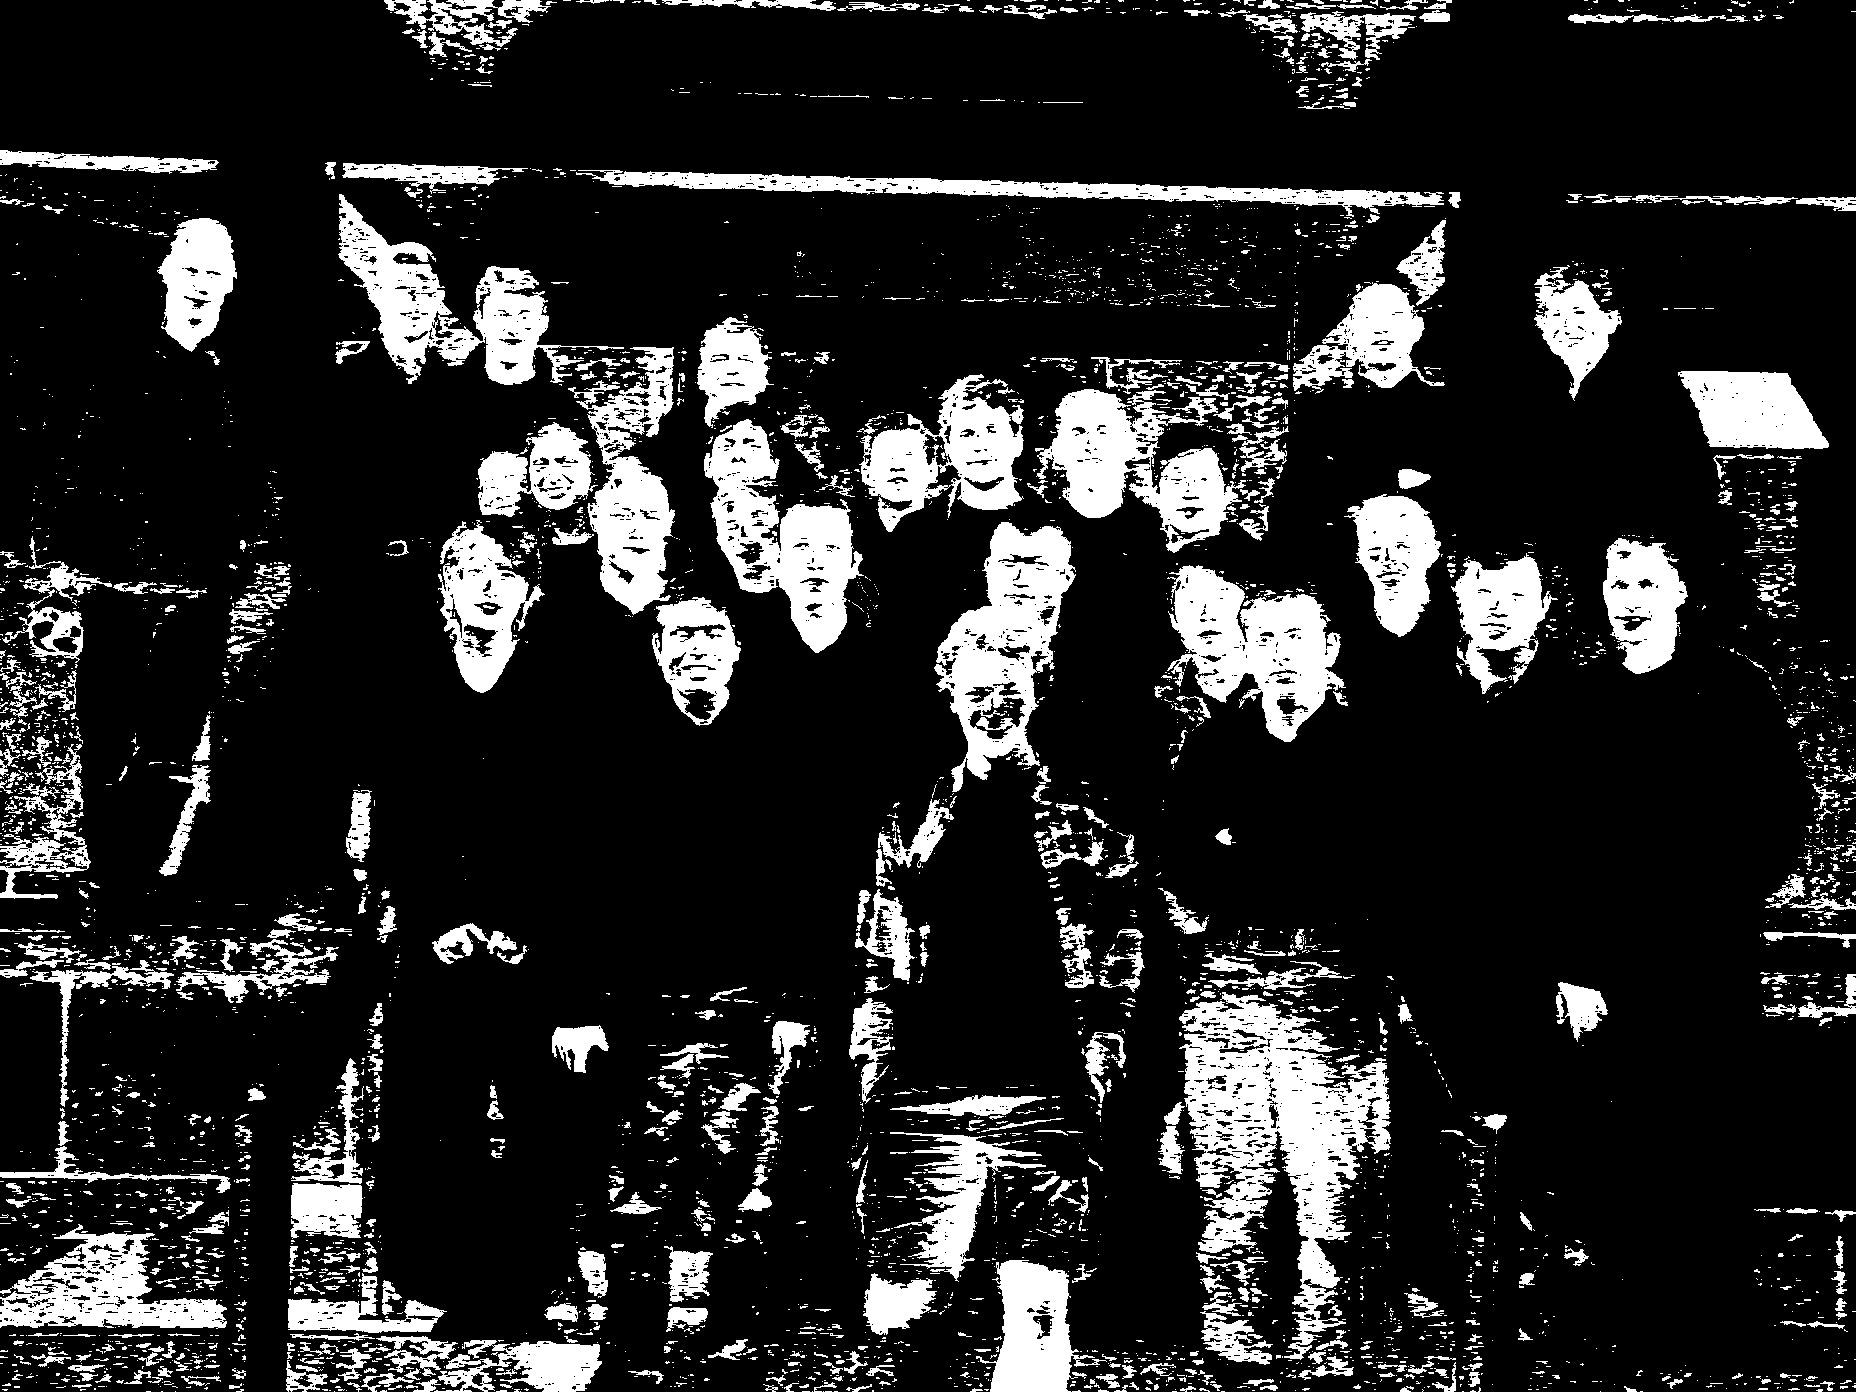
\includegraphics[scale=0.1]{classified3a-1}
    \newline
    \scriptsize
                    Figure 1: The resulting images from classification.
\end{center}
\begin{center}
    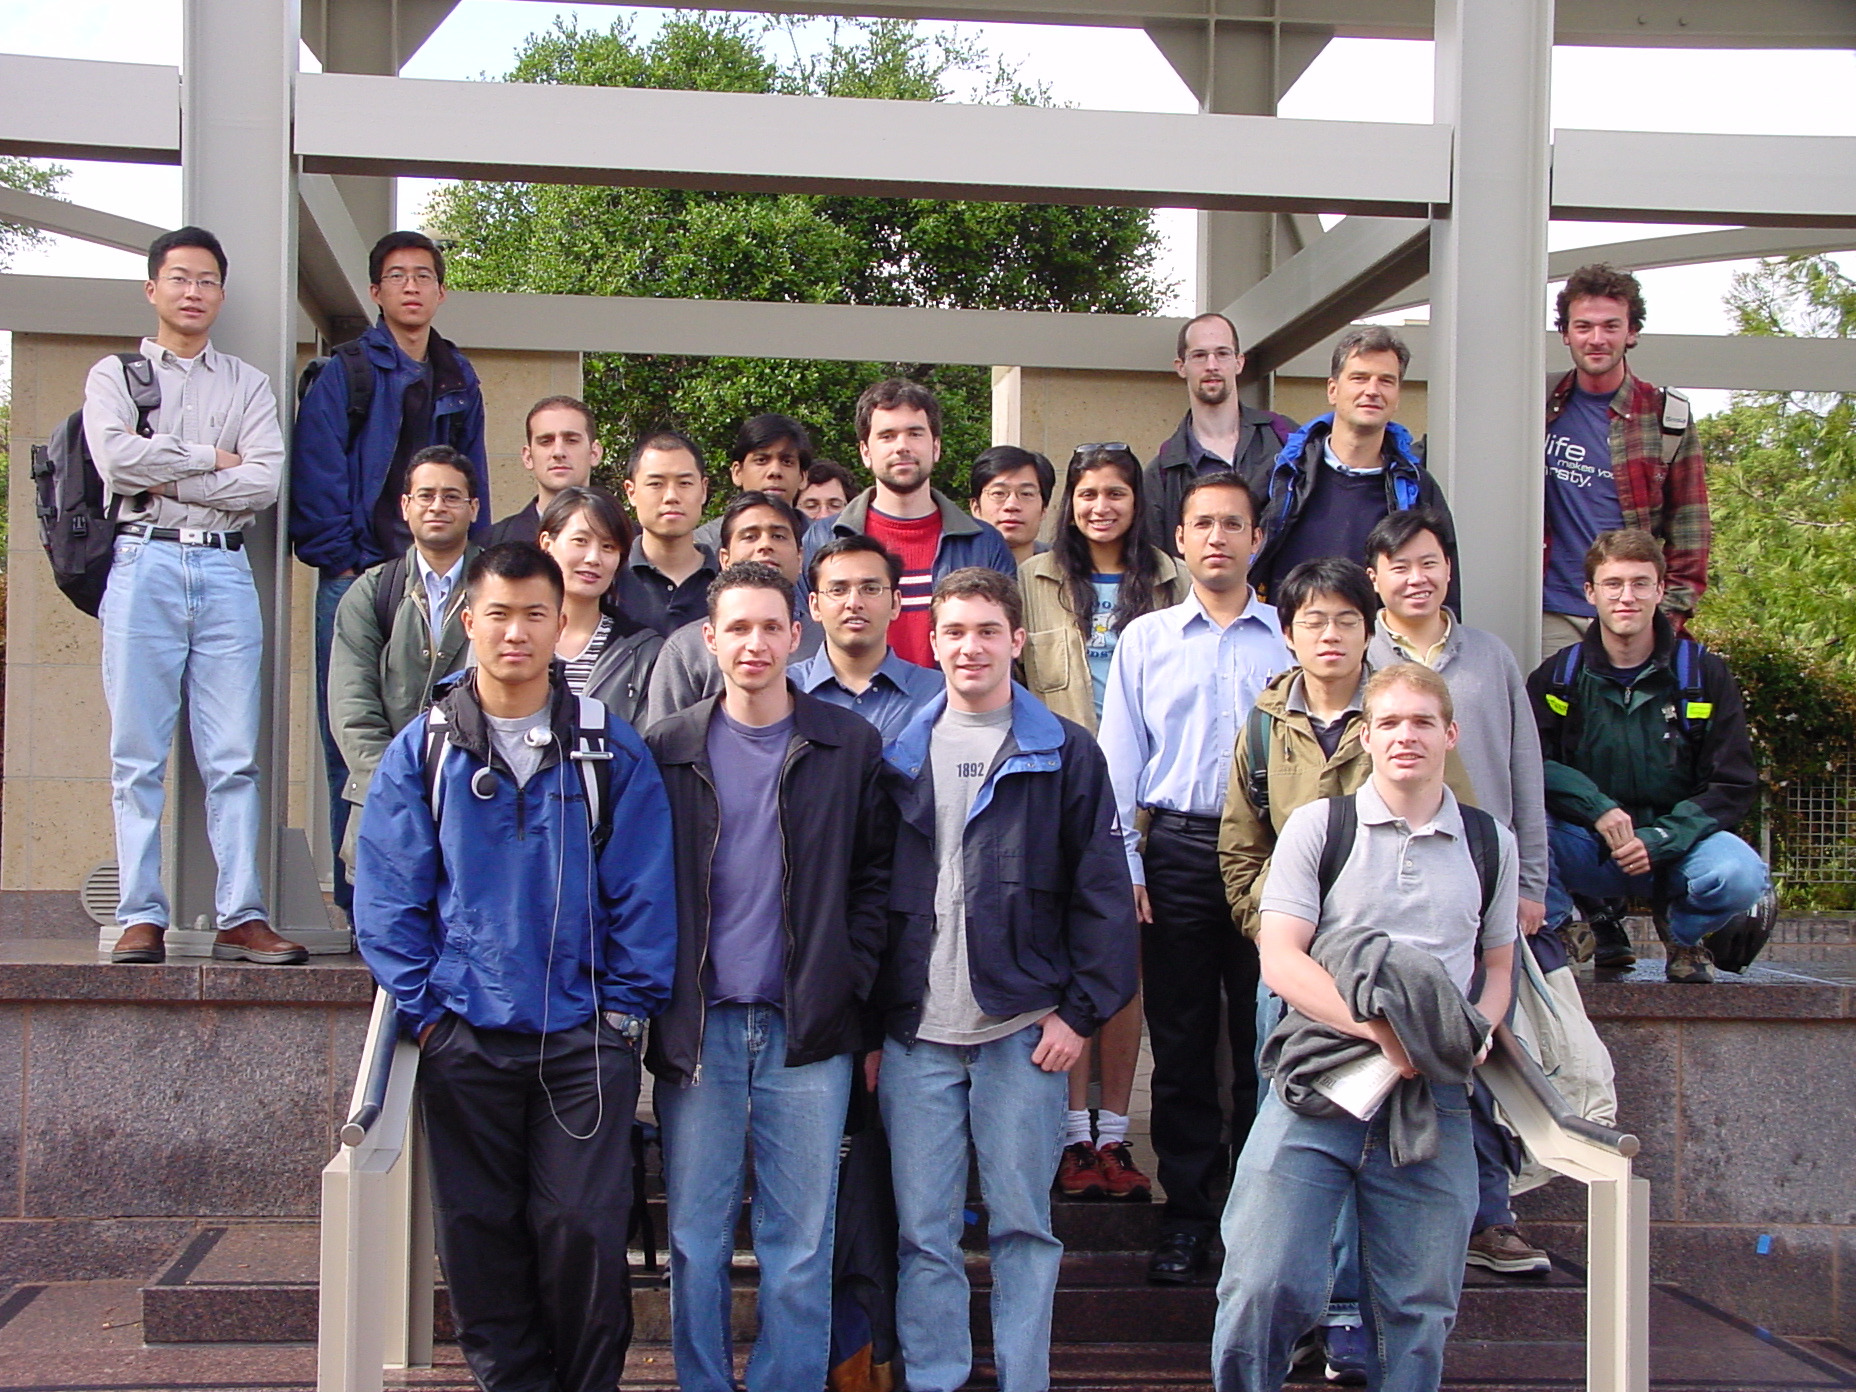
\includegraphics[scale=0.1]{Training_6}
    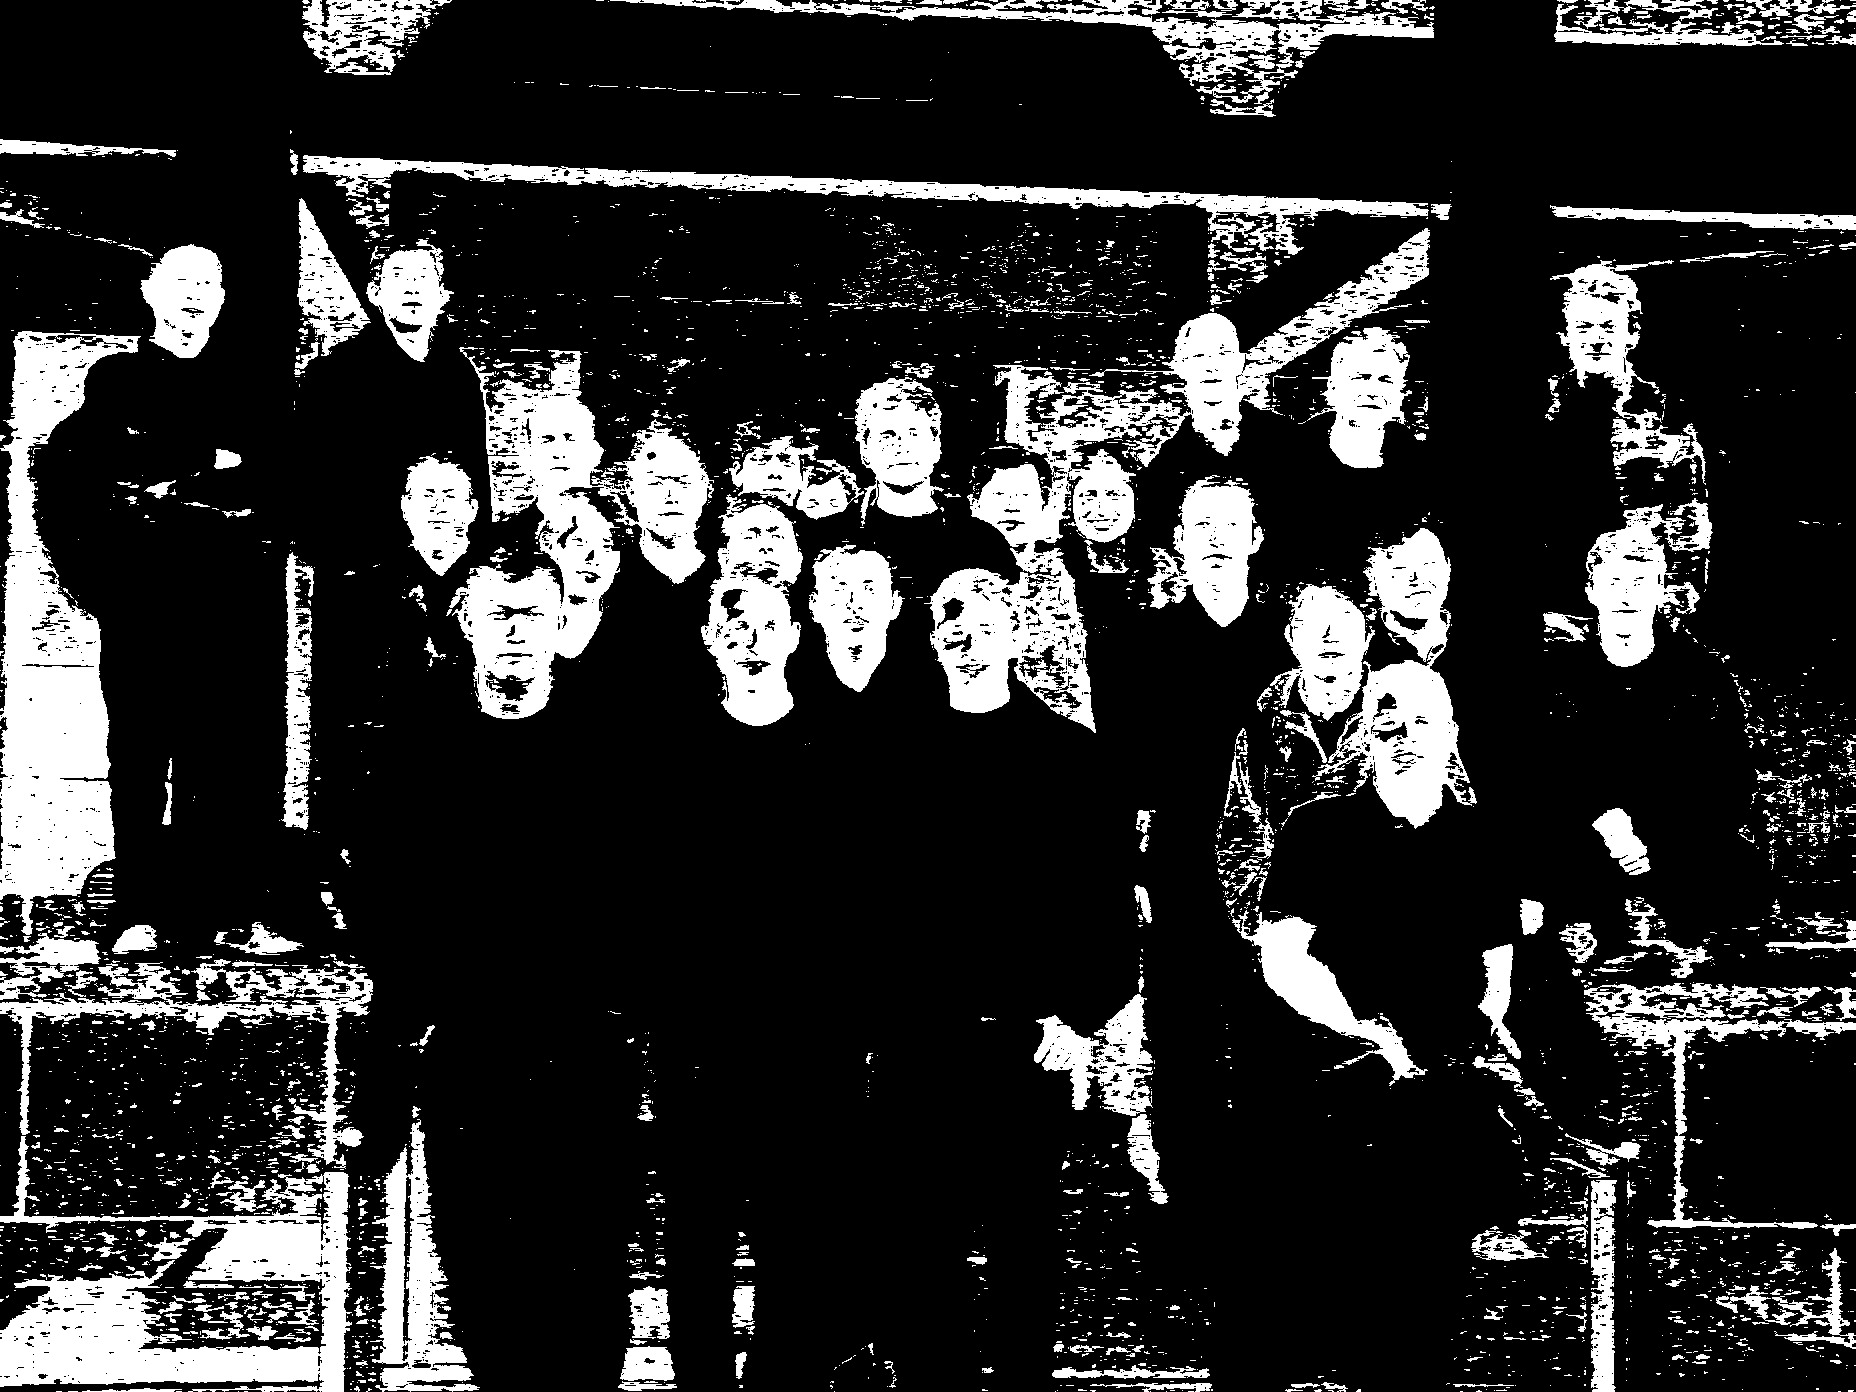
\includegraphics[scale=0.1]{classified3a-2}
    \newline
    \scriptsize
                    Figure 2: The resulting images from classification.
\end{center}


            \item[\textbf{b.}] The same experiment is repeated, now using the YCbCr color space. This produces slightly different optimum thresholds and classification results. Figures 3 and 4 show the results for the YCbCr color space.

    (insert other classification images here)

        In addition, ROC curves were generated for all four cases. Figure 3 shows the resulting ROC curves. The specific values for FP and FN are stored in ROC3a-1.csv, ROC3a-2.csv, etc.

    \begin{center}
    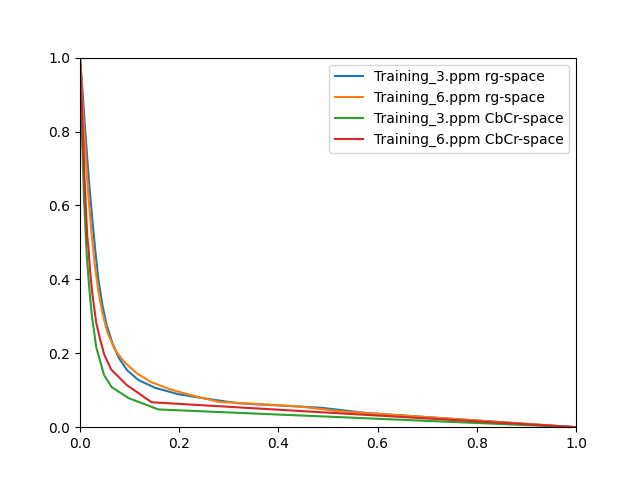
\includegraphics{ROC}
    \scriptsize
                    Figure 3: The ROC plot of the classification.
    \end{center}

        \end{enumerate}

\end{enumerate}


\end{document}

